

\documentclass{standalone}
\usepackage{pgfplotstable}
\usepackage{xintexpr}
\pgfplotsset{compat=1.12}

\begin{document}
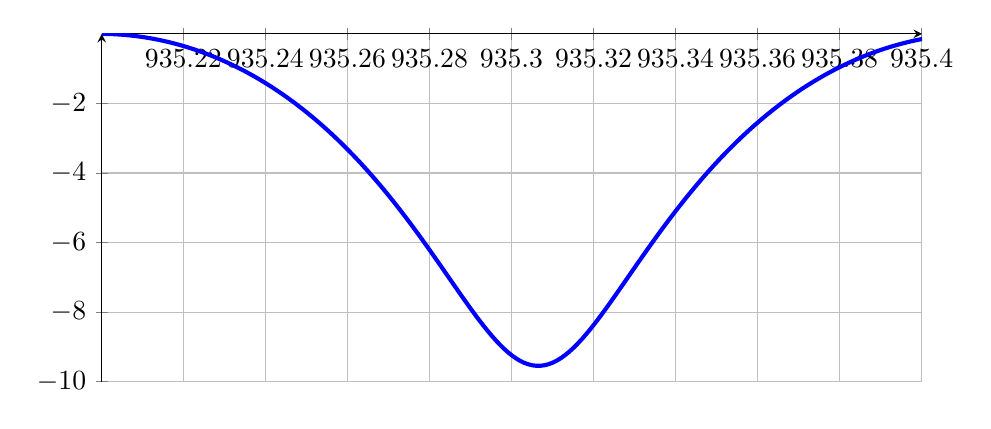
\begin{tikzpicture}
  \begin{axis}%
    [grid=both,
    log ticks with fixed point,
     width=12.0cm,
   height=6cm,
            % scale only axis,
     xmin=935.2, xmax=935.4,
    ymin=-10, ymax=0,
    domain=935.2:935.4,
    samples=1305,
     axis lines=middle,
     % enlargelimits={abs=0.2}
    ]
    \addplot+[mark=none, line width = 1.5] coordinates {%
      \xintthecoords% (converts x1,y1,x2,y2,... into (x1, y1) (x2, y2)...
                    %  format, as expected by "coordinates")
      \xintfloatexpr 
          seq((x,20*log10(abs((((sqrt(4*cos(((100*3.14159*x)/(3)))*cos(((20*3.14159*sqrt(41)*x)/(3)))+4*sin(((100*3.14159*x)/(3)))*sin(((20*3.14159*sqrt(41)*x)/(3)))+5))/(2)))/(1.5)))), x=935.2..[0.001]..935.4)
          % works with xint float engine
          % because exponent is integer (or half-integer)
      \relax
    };
    % \addplot[domain=-1:3,samples=50,smooth,red] {cos(deg(pi*x))};
  \end{axis}
\end{tikzpicture}
\end{document}
% \begin{tikzpicture}
%     \begin{semilogyaxis}
%         [
%            log ticks with fixed point,
%            width=12.0cm,
%            height=6cm,
%             scale only axis,
%             xmin=935.2, xmax=935.4,
%             ymin=1e-1, ymax=2,
%             grid=both,
%             domain=935.2:935.4,
%             samples=1400,
%             xlabel={Frequency: $f$},
%            ylabel={$|H(f)|$},
%            % label style={% erst nach Option axis lines verwenden
%            %  at={(ticklabel cs:0.5)},anchor=near ticklabel,sloped},
%         ]
%         \addplot+[mark=none, line width = 1.5] {abs(sqrt(4*cos(((100*pi*x)/(3)))*cos(((20*pi*sqrt(41)*x)/(3)))+4*sin(((100*pi*x)/(3)))*sin(((20*pi*sqrt(41)*x)/(3)))+5))/(2)/1.5}; 
%     \end{semilogyaxis}        
% \end{tikzpicture}
\end{document}

20*log10(abs((((sqrt(4*cos(((100*pi*x)/(3)))*cos(((20*pi*sqrt(41)*x)/(3)))+4*sin(((100*pi*x)/(3)))*sin(((20*pi*sqrt(41)*x)/(3)))+5))/(2)))/(1.5)))


((abs(w_t)*sqrt(4*cos(((100*pi*x)/(3)))*cos(((20*pi*sqrt(41)*x)/(3)))+4*sin(((100*pi*x)/(3)))*sin(((20*pi*sqrt(41)*x)/(3)))+5))/(2))
((abs(w_t)*sqrt(4*cos(((100*pi*x)/(3)))*cos(((20*pi*sqrt(41)*x)/(3)))+4*sin(((100*pi*x)/(3)))*sin(((20*pi*sqrt(41)*x)/(3)))+5))/(2))